% Sistema de nivel: dos tanques en cascada
\documentclass[border=5pt]{standalone}
\usepackage{tikz}
\usetikzlibrary{arrows.meta}
\begin{document}
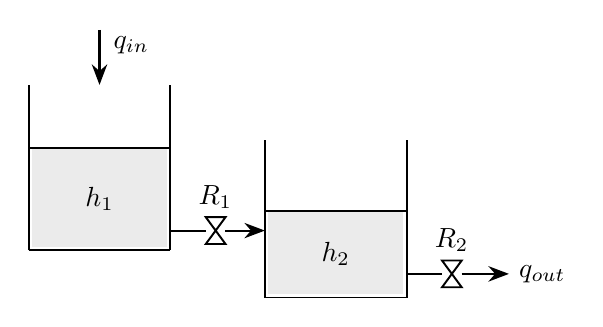
\begin{tikzpicture}[>={Stealth[length=2.6mm]}, line width=0.7pt]
  % entrada
  \draw[->, line width=1pt] (0.9,3.4) -- (0.9,2.7);
  \node[right] at (0.95,3.2) {$q_{in}$};
  % tanque 1
  \draw (0,0.6) -- (0,2.7) (1.8,0.6) -- (1.8,2.7) (0,0.6) -- (1.8,0.6);
  \fill[black!8] (0.04,0.64) rectangle (1.76,1.9);
  \draw (0,1.9) -- (1.8,1.9);
  \node at (0.9,1.25) {$h_1$};
  % valvula R1
  \draw (1.8,0.85) -- (2.25,0.85);
  \draw (2.25,0.68) -- (2.5,1.02) -- (2.25,1.02) -- (2.5,0.68) -- cycle;
  \node[above] at (2.37,1.0) {$R_1$};
  \draw[->] (2.5,0.85) -- (3.0,0.85);
  % tanque 2 (mas bajo)
  \draw (3.0,0) -- (3.0,2.0) (4.8,0) -- (4.8,2.0) (3.0,0) -- (4.8,0);
  \fill[black!8] (3.04,0.04) rectangle (4.76,1.1);
  \draw (3.0,1.1) -- (4.8,1.1);
  \node at (3.9,0.55) {$h_2$};
  % valvula R2
  \draw (4.8,0.3) -- (5.25,0.3);
  \draw (5.25,0.13) -- (5.5,0.47) -- (5.25,0.47) -- (5.5,0.13) -- cycle;
  \node[above] at (5.37,0.45) {$R_2$};
  \draw[->, line width=1pt] (5.5,0.3) -- (6.1,0.3);
  \node[right] at (6.1,0.3) {$q_{out}$};
\end{tikzpicture}
\end{document}
